\documentclass[10pt, compress]{beamer}

\usetheme{m}

\usepackage{booktabs}
\usepackage{minted}
\usepackage{graphicx}
\graphicspath{ {images/} }

\usepgfplotslibrary{dateplot}

\usemintedstyle{trac}

\title{Environnements de MOOC avec Docker}
\subtitle{Projet de fin d'études - VAP ASR}
\date{28 Janvier 2015}
\author{François Monniot \& Alexis Mousset}
\institute{Télécom SudParis}

\begin{document}

\maketitle

\section{Introduction}

\begin{frame}[fragile]
  \frametitle{Notre projet}

  Exemple de \emph{code} (du \alert{beau}) :

  \begin{minted}[fontsize=\footnotesize]{javascript}
// Instanciation du tracker
var tracker = new Tracker({distant: 'url'});

// On ecoute les evenements "onclick" sur les elements de classe "my-element"
tracker.on('.my-element').track('click');
  \end{minted}
  \begin{description}
    \item[PowerPoint] Meeh.
    \item[Beamer] Yeeeha.
  \end{description}
\end{frame}

\section{Présentation}

\begin{frame}[fragile]
  \frametitle{Qu'est-ce qu'un conteneur ?}
  \begin{center}
  
 
  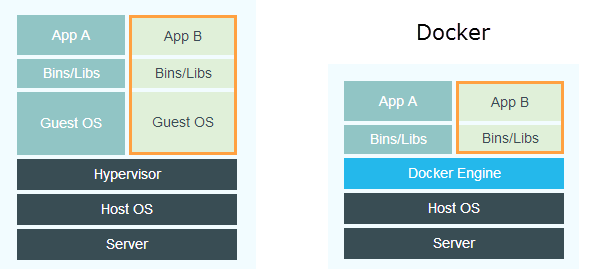
\includegraphics[scale = 0.5]{dockervsvm.png}
   \end{center}
\end{frame}

\begin{frame}[fragile]
  \frametitle{Develop, Ship and Run Any Application, Anywhere}
  Qu'apporte Docker ?
  \pause
  \begin{itemize}[<+- | alert@+>]
  \item Workflow intégrant tout le cycle du vie de l'application
  \item Rapide à créer, déployer et exécuter
  \end{itemize}
  \pause
   Comment ?
   \pause
  
\begin{itemize}[<+- | alert@+>]
  \item Docker Engine (démon + client)
    \begin{itemize}[<+- | alert@+>]
      \item Conteneurs jetables
      \item Images : layers, AUFS, versionning
      \item Volumes
      \item Liens
    \end{itemize}
  \item Docker Hub
  \begin{itemize}[<+- | alert@+>]
      \item Contient des images
      \item Images officielles
      \item Images publiques
      \item Images privées
    \end{itemize}

\end{itemize}
\end{frame}

\section{Cas d'utilisation}

\section{Démonstration}

\plain{Questions ?}

\end{document}
